\section{Significance of the Topic}

    \begin{itemize}
        \item
        "Mobile devices, such as smartphones and tablets, have become increasingly important in ourdaily life. These mobile devices with wireless technologies are also playing an important rolein teaching and learning (Gikas and Grant, 2013), as they serve as a virtual platform forlearners to engage with their learning activities in a more spontaneous, personal, informal,contextual, portable, ubiquitous and pervasive way. These unique characteristics andconvenience brought by mobile technologies serve as a bridge between the formal and informal learning, as learning has become an integral part of students’daily activities(Kukulska-Hulme and Traxler, 2005)." \cite{Mobile_Apps_Between_Hong_Kong_and_Japan}
        \item
        Almost everyone today uses a smartphone. Smartphone users are especially common in younger individuals, ergo college students. I can barely walk across campus without avoiding at least one person staring at their phone, ignoring the world around them. "Many libraries provide mobile app services because of the rapid increase in smartphone users" \cite{undergrad_ma}. Simple tasks can be completed quicker on a smartphone, rather than a laptop or desktop device. "Although more search tasks were completed using the laptop, participants could complete most tasks when using the mobile app and required less time to do so" \cite{undergrad_ma}. So, if we are to implement specific features in such a way that the user experience is quick and satisfying, we could remove some need for physical attendance to the library.
        \item
        We live in a world where convenience is key. People expect answers to all of their queries, and expect these results instantaneously. This makes sense as "technologies have made communication and access to information very convenient and timely to the users from the comfort of their own home and office" \cite{mob_ph_app_aca_lib}. Therefore, the same paradigm can and should be applied to library applications.
        \item
        Recently, smart phones with iPhone in the lead experience a huge popularity and the number of smartphones in the market has increased considerably. The reason behind this popularity is the plurality of useful and fancy applications [6], also called Apps. Although apps may have the same functionality there are many ways of implementing them such JavaScript, HTML5, applets,widgets, etc. Seen from the developers, users and service providers it is both interesting and relevant to understand the differences in terms of architecture, underlying mechanisms and functionality. Further, it is crucial in the development and selection of mobile apps to know which paradigm is more suitable for a given type of applications or usage. This paper is aiming at shedding light on the current most popular mobile app paradigms and providing a fundament for appropriate selection of mobile app paradigms. The paper starts with reviewing the related works. Next, the different mobile app paradigms are explained in a comprehensive way. The core of the paper is the evaluation of the existing mobile app paradigms. To verify the evaluation a practical implementation is carried out. A mobile object recognition/visual search app is chosen and is developed using the two most promising paradigms, namely native app and HTML5 mobile app. Evaluation results are also thoroughly discussed. \cite{Mobile_App_Paradigms}
        \item
        A mobile native application or native app is an application specifically developed to execute on a specific device platform[7] and machine firmware, and cannot be used for other device platform without modifications. For example, apps developed for the iPhone run only on Apple devices. A native app could be a stand-alone app running on the mobile phone or consisting of a main component on the mobile phone communicating with network servers. To use native apps users must download them from app store and install them manually on their phones.\cite{Mobile_App_Paradigms}
        \item
        Mobile widgets represent lightweight, task-specific apps that leverage Web content [8]. Mobile widgets exploit web technologies, including HTML, CSS, JavaScript and XML. Widgets will be executed within a runtime environment known as widget engine (e.g. Opera, Nokia WRT, Samsung TouchWiz and Yahoo!Blueprint). Different types of widgets need different widgets engines to execute. Like native app, a mobile widget could be a stand-alone application running on the mobile phone or consisting of a main component on the mobile phone communicating with a specific network server.\cite{Mobile_App_Paradigms}
        \item
        Mobile Web application is a good paradigm to deliver information and service to mobile phone. A mobile Web app enables information processing functions to be initiated remotely on Web server. The three-tiered architecture [9] is the most popular Web app architecture, which consists of thin client layer (mobile devices), application layer (Web server) and database. \cite{Mobile_App_Paradigms}
        
        \item
        HTML5 is specified by W3C to create a standard consisting of a set of features that can handle all the tasks that the current technologies (e.g. Adobe System Flash, Apple Quick Time and Java Oracle FX) are doing in a mobile Web apps. In the same way as mobile Web apps, HTML5 web app can have a threetiered architecture where demanding processing can be carried out remotely on the Web servers. Additionally, HTML5 supports newer mobile technologies, such as Geolocation [10] and Scalable Vector Graphic [16]. The new features of HTML5 that benefits mobile Web apps include: Canvas [11], video tags [12], location-based services [13], working offline [14] and Web workers [15]. \cite{Mobile_App_Paradigms}
        \item
        4. EVALUATION CRITERIA In order to really assert which mobile application paradigms are better it is necessary to consider the viewpoints of all the involved players, namely developer, user and service provider. We deduced the evaluation criteria as follows:
        x Developer’s viewpoint
         x Ease of developing:
            o  Programming language: This sub-criterion tells both about the simplicity and the popularity of the programming language.
            o Software Development Kit (SDK):
                a Applicability: This sub-criterion relates the applicability and accessibility of the SDK.
                a Specifications and tips: This sub-criterion is about the quality of documents accompanied with the SDK.
                a Download installation and configuration: These sub-criterion shows how straightforward to download install and configure the SDK on our development environment.
            o Support from community: This sub-criterion is about how much help developers could receive from community (e.g. tutorials, development tools and troubleshooting).
        x Ease of coding:
            o IDE capability:
                a Code editor: This sub- criterion is about the qualification of the IDE adopted for the app development. A good code IDE will provide immediate feedback with error messaged and warnings, quick fix feature, content assistant and a good guidance document.
                a User interface builder: This sub-criterion shows how robust the adopted user interface builder is. A powerful user interface builder will have instantly viewable and drag-and-drop capabilities, and other features reducing the workload of developers to create an attractive user interface.
            o User interface: This sub-criterion shows how straightforward it is to build an attractive and adaptive user interface.
            o Device’s interaction:
                a Hardware: This sub-criterion describes how easy it is to access device’s hardware, such as camera, storage and WLAN card.
                a Built-in apps: This sub-criterion shows how effective it is to adopt different built-in apps on devices, such as camera, phonebook and photo gallery apps
            o Web service interaction: This sub-criterion is to evaluate the ease of using a Web service, such as Google Map, Facebook and IQEngine.
        x Ease of debugging: This sub-criterion tells about how powerful and applicable the debugging tools are. A robust debugging tool will help manage break point, trace object value through the code and identify unexpected bugs.
        x Ease of testing:
            o Emulator: This sub-criterion show how effective is the testing of apps on an emulator. A powerful emulator will run fast and support as many device’s features as possible, such as GPS, camera, and accelerator.
            o Real device: This sub-criterion show how easy is the testing of apps on a real device.
        x Ease of deploying and updating: This criterion relates how straightforward it is to deploy and update an app onto a real device.
        x Ease of distribution:
            o Compatibility: This sub-criterion shows how easy it is to distribute an app to multiple platforms.
            o With app store: This criterion shows how easy it is to distribute an app via app store.
            o Without app store: This criterion relates the possibility of distributing an app without the app store. 
        x Application types:
         o Application using device’s capability: This subcriterion evaluates the possibility of apps to use device’s hardware such as camera, keypad and GPS.
            o Application using server’s capability: This subcriterion describes the possibility of apps to use server’s capability such as storage and processing.
        x Powerful APIs and libraries: This criterion shows the robustness and the popularity of the APIs and libraries that developers can use to build mobile apps.
        x Payment possibilities: This criterion relates the possibility to earn revenues from the sale of app.
        x User’s viewpoint
        x Ease of use:
            o Performance: This sub-criterion presents the response time of the app in milliseconds. The shorter time we use the better the app performs.
            o User interface: This sub criterion evaluates how attractive, adaptive and responsive the app is.
            o Operation: This sub-criterion shows the ease of use of app. For example, it evaluates how to start the app and how to navigate between the functionalities of the app.
        x Functionality
            o Working offline: This sub-criterion evaluates the capability of working offline of the app.
            o Accessing device’s hardware: This sub-criterion describes how effectively the app can access device’s hardware (e.g. camera, GPS and storage).
        x Installation and update
            o Compatibility: This sub-criterion shows the compatibility of the app and how easy to install it on different mobile platforms.
            o Downloading, installing and updating: This subcriterion shows the simplicity of downloading, installing and updating the app on mobile phones.
        x Service/content provider viewpoint
        x Content management
            o Content presentation: This sub-criterion shows how complicated it could be to present the content on a mobile phone due to the limitation on screen’s size and computing resource.
            o Content delivering: This sub-criterion evaluates the ease of delivering the content to mobile phones.
        x Administration
            o Security: This sub-criterion evaluates the effort of content provider to secure their service (e.g. authentication, confidentiality and integrity).
          o Maintenance: This sub-criterion shows the ease of hosting, managing, updating and maintaining the app.
        x Distribution: This sub-criterion shows how easily service/provider distributes their apps to end users.\cite{Mobile_App_Paradigms}
        \item
        With the prevalence of smartphones, mobile apps have seen widespread adoption. The number of apps in both Apple App Store and Google Play has surpassed the two million mark in 2016 and billions of downloads [6, 20], which makes mobile apps a big industry. Recent studies [4, 44] reported that the global mobile app revenues amounted to 41.1 billion US dollars in 2015 and the app economy could double in size to more than 100 billion dollars by 2020. At the same time, the latest estimates [32] indicate that there are 12 million mobile app developers worldwide, representing more than half of the total community, and almost half of app developers focus their attention on the Android platform, which makes mobile app market a very competitive environment. A large mount of research work have focused on the mobile app ecosystem. \cite{Mobile_App_Ecosystem}
        \item
        App developers are the cornerstone of the mobile app ecosystem. Besides large corporations such as Google and Facebook, individual developers and small companies also play important roles in the app development field. However, few studies have focused on app developers, and very little is known about this part of the mobile app market ecosystem.\cite{Mobile_App_Ecosystem}
        \item
        Cravens et al. [14] explored the demographic and business model of app developer based on a web-based survey of 352 developers. Balebako et al. [8] have explored how app developers make decisions about privacy and security. Their findings suggested that smaller companies are less likely to demonstrate positive privacy and security behaviors. BelloOgunu et al. [9] developed plugins for the Eclipse IDE to guide developers on the set of required permissions when creating Android applications. Websites such as App Brain [5] have published basic statistics of app developers. However, no previous work has detailed analyzed the distribution of app developers, the difference in the practices of various kinds of developers and the privacy behaviors of app developers in large scale.\cite{Mobile_App_Ecosystem}
        \item
        The popularity of mobile devices, i.e., smart-phones and tablets, has been rapidly growing. These mobile devices run mobile apps. Mobile apps are small software applications that are intended to achieve specific functionalities. For example, some mobile apps are used for gaming; others are used for everyday banking.\cite{Challenges_in_Mobile_Apps}
        \item
        The software engineering research community has over the past few decades made giant strides in observing, understanding, and improving software that is run of desktop devices and backend servers. However, mobile apps are very different from such software. One key difference is that mobile apps are often distributed through centralized market places called “App Stores”. In such markets even small team of developers can be highly successful. A considerable number of apps are very small in size and sometimes tends to follow no particular design principle.\cite{Challenges_in_Mobile_Apps}
        \item
        We see mobile versions of websites. They are often stripped down versions of their full desktop counterparts. "It is basically a short version of large website that is designed and optimised for viewing on mobile devices... The general purpose of a mobile website is to make the content or at least a subset of the content, available to the users". There are some advantages to developing a mobile library website, such as that it "only needs to be developed once, unlike native applications that need to be developed for each specific mobile platform. Another advantage of mobile websites is that they are easier to maintain than native applications, the third advantage of developing mobile library website is that it is more cost effective than developing a native application" \cite{misodi}. All of these are positives. And it makes sense for us to develop a web application rather than a native application.
        
    \end{itemize}

    
   

\section{Known and Unknowns}
    \begin{itemize}
        \item
        It may be easy to throw together a quick application, but developing an app that people want to use is another beast entirely. "The adoption of mobile apps as an emerging format within the Libraries’ collections necessitates a varied outreach strategy that endeavors to make apps accessible and approachable" \cite{saragossi_costello_kasten_2018}. It may be easier "achieved through hands-on workshops or the creation of robust resources for online users" \cite{saragossi_costello_kasten_2018}. This is why designed and surveyed students and faculty.
        
        \item 
        Techniques ranging from the manual inspection to
        automated static and dynamic analyses are commonly employed to
        identify security vulnerabilities prior to the release of the software.
        However, none of these techniques is perfect, as static analysis is
        prone to producing lots of false positives and negatives, while dynamic analysis and manual inspection are unwieldy, both in terms
        of required time and cost. \cite{MiningMobileApp}
        
        \item
        The effectiveness of mobile learning is undoubted, and conceptions of mobile learninghave been explored and documented in the education and information systems (ISs)literature. Judy Brown, the Director of Academic Advanced Distributed Learning (ADL)Co-Lab suggested that there will be one global mobile campus, while the devices are rapidlyevolving and capabilities are increasing, which will improve the learning quality andeducation in within 10–20 years, starting from 2005 (UNESCO, 2005). While the currentcomputing power of mobile devices becomes comparable to desktops, a key factor to enable itto take off is whether learners would like to use this technology to assist and engage inlearning activities, such as using the mobile devices to access library services. The latterfactor is, indeed, affected by a learner’s perception of the usefulness of such technology.Accessing online library services has been widely considering an essential learning activityacross all disciplines at different study levels, especially under the wide adoption of inquiry-based learning in higher education (Dougherty, 2010). \cite{Mobile_Apps_Between_Hong_Kong_and_Japan}
        
        \item 
        "TableIIdemonstrates that the participants spent differentamounts of time to complete different tasks; the participants spent more time completing taskswhile using the laptop than that they did while using the mobile app. The results indicated thatthe participants spent longer time completingTask 4 (a subject search) than the other threetasks. For Task 1, participants spent twice the time to complete the task while using the laptop(01:55) than they did while using the mobile app (00:53). Similar findings were noted for Task 2." \cite{given_one}
    \end{itemize}
    
    
\section{Current Models in This Field of Study}
    \paragraph{}
    A 2018 study performed by Dr. Ali Mansouri and Nooshin Soleymani, titled "Accessing mobile application components in providing library services," aimed to investigate the necessarily features for a library mobile application. The research was performed at the University of Isfahan, known for science, humanities, and engineering. Dr. Ali Mansouri, a professor at the university in the Department of Knowledge and Information Science, lead this study, and others relating to information management and library and information science. Nooshin Soleymani is also credible, with her masters in Library and Information Science.
    \begin{figure}[H]
        \centering
        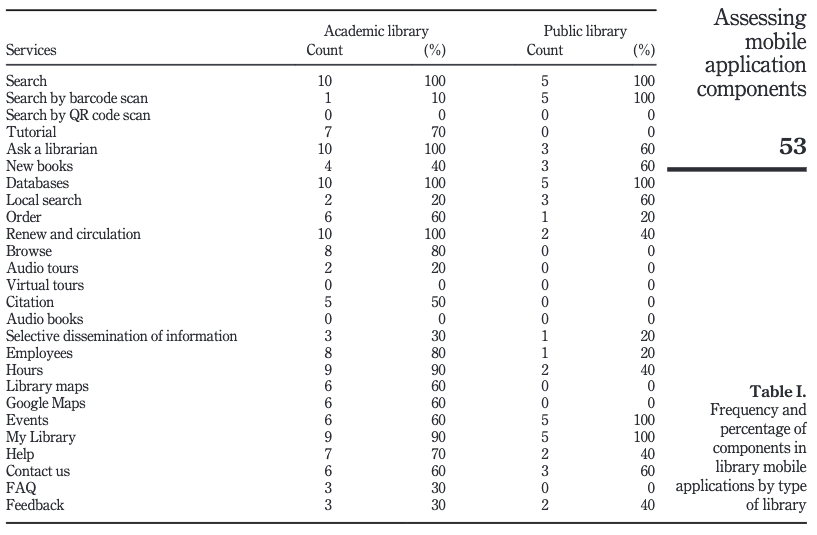
\includegraphics[width = \textwidth, height = \textheight, keepaspectratio]{assets/img/accessing_mobile_application_components_table_1.png}
        \caption{Frequency and percentage of components in library mobile applications by type of library \cite{mansouri_soleymani_asl_2019}}
        \label{fig:freq_and_per_comp_lib_mob_app}
    \end{figure}
    \paragraph{}
    The above (Figure ~\ref{fig:freq_and_per_comp_lib_mob_app}) is from Mansouri and Soleymani's study. In summary, it breaks down all services found in the library mobile applications they reviewed, and how often they were used. The "Public library" column is irrelevant in this report. This is a great example of a model for features that are used in the field already. We will break down all relevant features and provide comments on each.
    \paragraph{Search (by barcode/QR code scan)}
    We assume these features refer to a user's ability to search the library catalog. At the time of this writing, this is a feature we do not plan on implementing in the \appname app. However, it is an important one, as according to this study, all existing library apps reviewed had this features. We believe for a mobile app that is intended to be a replacement for a desktop website to be successful, it must provide the most common services provided by its desktop website counterpart.
    \paragraph{Tutorial}
    We assume this feature refers to a visual tutorial provided within the mobile app that teaches new users how to use said mobile app. The study found that 70\% of library mobile apps had this feature. A tutorial allows new users to get a better understanding of how to use a platform. Without a tutorial, many new users may be lost, therefore rendering the mobile app useless for them. As of this writing, we had not considered this feature, but have since taken it under consideration.
    \paragraph{Ask a librarian}
    We assume this feature refers to a user's ability to submit questions to a librarian. The study found all library mobile apps included this feature. We plan to implement a similar feature: the library chat.
    \paragraph{Audio books}
    We assume this features refers to a user's ability to search and listen to audio books. We have discussed this with our advisor, who says the WPI library has a lot of audio books in its database. As of this writing, we have dismissed the idea of implementing this feature. As this study shows, it seems that others have too. We do feel that this features would be interesting, but clearly, according to the study, there has been no adoption (among the study's data set).
    \paragraph{Hours}
    Straight-foward features that provides users with library hours. We plan on implementing this feature in the \appname app.
    \paragraph{Events}
    We assume this feature refers to a user's ability to view library events and/or a calendar. The study found that 90\% of library mobile apps have this feature. We plan on implementing it as well. If we are to produce a library mobile app with many other features, it is possible that users will prefer the app to the desktop website. It would be silly to not include such a useful feature such as a calendar of library events. Users should not have to use a separate service.
    \paragraph{FAQ/Feedback}
    It surprised us that only 30\% of library mobile apps have this feature. The whole point of this project is to provide students easier access to the WPI library's various services. As a team of four (including our advisor), it is impossible for us to make a perfect product. This would really apply to any team size because there is always some disconnect between what the developers think consumers want, and what the consumers actually want. We plan on implementing a platform for users of the \appname app to provide feedback on their experience.

    \begin{itemize}
        
        \item
        The use of mobile apps is increasingly widespread, and much effort is put into testing these apps to make sure they behave as intended.To reduce this effort, and thus the cost of mobile app testing, we propose AppTestMigrator, a technique that allows for migrating test cases between apps with similar features. The intuition behind AppTestMigrator is that many apps share similarities in their functionality, and these similarities often result in conceptually similar user interfaces (through which that functionality is accessed). Typical examples of this situation are apps in the same category, apps developed based on the same specification, and different versions of the same app. In all these cases, the burden of writing test cases can be reduced by migrating test cases written for an app to another, similar app. Given a test case for an app (source app) and a second app (target app), AppTestMigrator attempts to automatically transform the sequence of events in the test for the source app to events that can be consumed by the target app.\cite{Test_Migration}
        \item
        Mobile apps are used on a daily basis to perform a number of tasks such as reading the news, accessing social media, and shopping. It is therefore important to thoroughly test these apps, to gain confidence that they behave as intended when used in the field. Unfortunately, developing test cases for an app, as for any software system in general, is extremely expensive. We believe that the cost of testing mobile apps can be considerably reduced by considering similarities between apps and reusing test cases across similar apps. \cite{Test_Migration}
        \item
        We presented AppTestMigrator, a technique that aims to decrease the cost of app testing by leveraging the similarities between GUIs of different yet related apps and performing test migration—reusing and adapting test cases among such apps. AppTestMigrator can be used in all those situations in which different apps share similarities that result in conceptually similar GUIs. We implemented a prototype of AppTestMigrator that supports Android apps and tests written using the Espresso framework, and we have used our prototype to evaluate our approach on four randomly selected shopping list apps from the Google Play Store. We believe that our results, although still preliminary, show clear evidence of the potential usefulness of our approach. In future work, we will first perform additional experiments to validate our findings and guide future research. Second, we will extend the technique so that it can migrate test oracles (i.e., assertions), in addition to events. Finally, we will investigate large scale applications of our approach, in the context of a database of apps and tests for these apps. Developers could submit their apps to the database, which would analyze them, look for similar apps, migrate the tests from these apps, and return all the tests that were successfully migrated. If successful, this could result in a sort of store that operates in parallel to the app store. \cite{Test_Migration}
    \end{itemize}
    
    
\section{State of the Art}
    \begin{itemize}
    \paragraph{}
    Throughout the years, app development has improved in both efficiency, quality, and accessibility. As a result, library apps - as well as similar learning-based apps - have improved in these criteria congruently. One feature of modern day mobile applications is an emphasis integration with other relevant software. For example, in reference to the Libris CampusM Mobile App, an article writes: "The flexibility of the app enables it to be integrated with learning management systems such as Blackboard®, Canvas, and Moodle™" \cite{campusM}. 
    
    \paragraph{}
    \paragraph{}
        \item
        "The flexibility of the app enables it to be integrated with learning management systems such as Blackboard®, Canvas, and Moodle™" \cite{campusM}
        \item
        "Since the app runs on library-developed open-source software, feedback from academic users during the pilot program – currently running until August 31 – will also help develop and improve new functionality in the app, which will benefit all library users." \cite{NYU_Library}.
        \item
        "Since the app runs on library-developed open-source software, feedback from academic users during the pilot program – currently running until August 31 – will also help develop and improve new functionality in the app, which will benefit all library users." \cite{NYU_Library}.
        \item 
        "The behavior of smartphone apps is driven by input from
        sensors such as GPS, microphone, or camera", 
        "First, we fuzz (alter) the log in a semantically-meaningful way: by applying 
        principled transformations (e.g., changing GPS coordinates
        or navigation speed), a new input log is constructed, which
        represents a new test case. Second, we use the log captured
        in app A to test an app B which offers similar functionality,
        e.g., GPS navigation or image recognition"
        "For example, GPS allows apps such as Yelp to provide location-aware services; the camera allows image matching apps like Google Goggles to provide search-by-picture features; the Shazam app can help recognize an ambient song by using the microphone."
        \cite{FuzzyAndCross}
        \item
        With the unceasing advancement of mobile technologies, mobile devices developed rapidly. Thus, learning activities could be proceeded anytime and anywhere (Lai et al. , 2014). Wang et al. (2012) indicated that, with the popularization of 3G mobile technologies, more people gained access to internet to view web site, receive and send e-mails and read e-books with smartphones and tablet PCs on metro, bus or train. It could be inferred that learning activities no longer limit to classroom or scheduled time. By combining mobile devices and wireless technology, learning guidance and feedbacks could be given according to learners' learning situations and learning environment (Huang et al. , 2014).

        A number of libraries gradually sensed this trend and combined their services with mobile technology to created so-called Mobile Library or M-Library. In fact, the concept of Mobile Library or M-Library was brought up by scholars when PDAs were still in development. For instance, Janet (2009) adapted mobile technology and combined PDA with library orientation and collection search services. However, at that time, mobile devices and wireless technology were not mature and popular.
        
        "Recently, mobile technology combined with mobile devices has become an important information collecting channel. A greater number of students and teachers also use tablet PCs and smartphone to search for e-journals, e-books and other e-resources (Parsons, 2010). Therefore, numerous libraries introduced mobile technology in library services and developed mobile information systems compatible to mobile devices in order to allow their users quickly search for desired information (Wang et al. , 2012). This indicated that Mobile Library has become a vital resource for learners to acquire knowledge."
        "Ten participants reported that it was easier to search the library catalog using the laptop.They explained that they were familiar with the interface of web OPACs, and moreinformation was displayed on the computer screen than the tablet screen"
        "Some participants reported that they would use the smartphone app to search librarycatalogs when it was inconvenient to use laptops or desktop computers, such as on the bus or in classroom"
        \cite{given_one}
       
    \end{itemize}
    
\section{Relation to the Larger Problem Area}
    \begin{itemize}
        \item 
        "The open-source community is helping to rapidly advance mobile Web application development. To date, no less than eighteen different mobile frameworks exist just for the iPhone. Yet few mobile Web developers know of them and their rich user interface capabilities and smart device features. MobiOne is introducing Community Insights, an integrated feature that brings together real time news and information about mobile Web frameworks with numerous examples that can be instantly loaded into the MobiOne iPhone and Palm Pre emulators for evaluation. "This time next year we expect the mobile Web to have matured significantly as smartphones get cheaper and more diverse, and desktop developers spend more energy creating applications for the computer in your pocket," said Maher Masri, president and CEO of Genuitec. "Mobile devices are becoming more prevalent and as the market grows, software developers will be armed for success with powerful tools like MobiOne.""\cite{MobiOne}
        
        \item
        There exists a trend towards mobile computing. "Gradually, many libraries sense this trend and start to ponder on methods of providing innovative services by using mobile technology". Mobile innovative services of library means that a library utilizes mobile technology to allow is readers view,search and obtain library services without being limited by time and place (Chang,2013) \cite{pu_chiu_chen_huang_2015}. In summary, libraries are attempting to offer mobile applications for their services. We want to do exactly that. We want an application that students can use wherever and whenever to access library services.
        
        \item
        "Recently, mobile technology combined with mobile devices has become an important information collecting channel. A greater number of students and teachers also use tablet PCs and smartphone to search for e-journals, e-books and other e-resources  (Parsons,  2010).  Therefore,  numerous  libraries  introduced  mobile technology in library services and developed mobile information systems compatible to mobile devices in order to allow their users quickly search for desired information(Wanget al., 2012). This indicated that Mobile Library has become a vital resource for learners to acquire knowledge" \cite{pu_chiu_chen_huang_2015}.
        \item
        Found in a study by a team from San Agustin University's Computer Science department in Peru, and among 163 surveyed students, those students mostly utilize academic apps that assist in making their academic workload easier and more efficient to handle. These such apps include: GeoGebra, Mathway, Kahn Academy, Duolingo, Symbolab, and numerous others. As we delve into the concept of creating a more ease of access system for academic resources here at WPI, this study shows just what students are wanting from mobile apps, convenience.\cite {Educational_Apps}
    \end{itemize}
    
    
    
\section{Additional Mobile Academic Library App Research}
        \subsection{Harvard University}
            \paragraph{}
            Harvard's library app, Harvard Library, featured a minimalist home screen with the school logo in the upper-right hand corner, a help button in the lower-left, a 'login' feature in the lower right, and a circular 'start' button in the center. The screen featured only three colors; white, black and crimson red. Clicking the 'start' button pulled up the same login screen that clicking the 'login' button pulled up.  Unfortunately, we were not able to further explore this mobile app because we do not have account affiliated with the University.
        \subsection{Salisbury}
            \paragraph{}
            Sailsbury Universitie's Library app, SU Libraries, featured a noticeably less minimalist design than Harvard's, and had a more unrefined look.  Fortunately, we were able to access the applications features, however. The home screen included a search bar, and nine features: "Library Hours", "Research Help", "Room Reservations", "Self Checkout", "SU Libraries MakerLab", "Device Availability", "Building Maps", "Helpful Links" and "Contact Information". It also contained a bar at the bottom with five navigation options: "Home", "Library News", "Chat", "My Card" and "About". Additionally, there was a link to the libraries social media accounts.
            \paragraph{}
            The "Library Hours" feature lead to a screen with minimal interactivity. The screen contained the opening and closing times for all days from the current day to approximately three months in advance. The "Research Help" feature took the user to a page with a somewhat similar layout; a page in which you could scroll downward, containing the subjects in which you could get research help. This page, however, was interactive. The user could click on each subject option, taking them to a page with information about who to contact, and how to contact them, if they are seeking research help in that specific area.  The "Study Room Reservations" feature as well as the "Devise Availability" feature has a similar layout to these two.
            \paragraph{}
            The "Building Maps" feature lead to a page containing the layout of each floor of the building. The only interactivity on this page was the option to click on any of the diagrams for an enlarged view of the diagram. 
            \paragraph{}
            The "SU Libraries MakerLab" feature took the user to a page which seemed functioned like an app in and of itself. The page it took the user to contained a variety of features relating to the Maker Lab. Such as a feature displaying the time its open for today as well as a feature displaying which days it is open. It also had a feature containing taking the user to a page with the Maker Lab policies, a feature allowing users to make an appointment in the maker space, and finally the contact information for the maker space. 